\documentclass[utf8]{beamer}
\usepackage{listings}
\usepackage[russian]{babel}
\usetheme{Malmoe}
\title{Передача данных на физическом уровне (II)}
\author {Компьютерные сети и протоколы}
\date{Лекция 3}
\begin{document}
%--------------------------------------------------------------------------------
\begin{frame}
\titlepage
\end{frame}
%--------------------------------------------------------------------------------
\begin{frame}
\frametitle{Материалы прошлой лекции}
\begin{block}{Стандартизация в области телекоммуникаций}
\begin{itemize}
 \item Международные организации по стандартизации
 \item Стандартизация Интернета
\end{itemize}
\end{block}
\begin{block}{Теоретические основы передачи данных}
\begin{itemize}
 \item Теорема Котельникова;
 \item Понятие о модуляции;
 \item Теорема Найквиста, OFDM в качестве примера.
 \item Теорема Шеннона
\end{itemize}
\end{block}
\end{frame}
%--------------------------------------------------------------------------------
\section{Проводные среды передачи информации}
%--------------------------------------------------------------------------------
\subsection{Витая пара}
%--------------------------------------------------------------------------------
\begin{frame}
\frametitle{Витая пара}
\begin{center}
\includegraphics[width=0.4\textwidth]{pics/UTP.png}
\end{center}
\begin{itemize}
 \item Скрутка позволяет снизить ЭМ-взаимодействие между двумя соседними парами
 \item Полоса пропускания зависит от диаметра и длины провода
 \item Полоса пропускания до 500 МГц
 \item Выделяют различные типы витых пар (наличие/отсутствие экранировки)
\end{itemize}
\end{frame}
%--------------------------------------------------------------------------------
\subsection{Коаксиальный кабель}
%--------------------------------------------------------------------------------
\begin{frame}
\frametitle{Коаксиальный кабель}
\begin{center}
\includegraphics[width=0.4\textwidth]{pics/coax.png}
\end{center}
\begin{itemize}
 \item Лучшая по сравнению с витой парой экранировка
 \item 50-Омный кабель -- цифровая передача
 \item 75-Омный кабель -- аналоговый сигнал
 \item Полоса пропускания -- до нескольких ГГц
\end{itemize}
\end{frame}
%--------------------------------------------------------------------------------
\subsection{Линии электропитания}
%--------------------------------------------------------------------------------
\begin{frame}
\frametitle{Линии Электропитания}
\begin{itemize}
 \item [$+$] Готовая инфраструктура
 \item [$+$] Отсутствие лишних проводов у мультимедийных устройств
 \item [$-$] Электропроводка не приспособлена для передачи высоких частот
 \item [$-$] Без скручивания электропроводка -- большая антенна
 \item [$-$] Помехи в момент включения приборов
\end{itemize}
\begin{block}{Существующие решения}
\begin{itemize}
 \item Существуют решения со скоростью передачи данных до 100 МБит/с
 \item Отсутствие на сегодняшний день международных стандартов
 \item WiFi -- дешёвая альтернатива
\end{itemize}

\end{block}

\end{frame}
%--------------------------------------------------------------------------------
\subsection{Волоконная оптика}
%--------------------------------------------------------------------------------
\begin{frame}
\frametitle{Волоконная оптика}
\begin{itemize}
 \item Минимальная вероятность ошибки на бит $\approx10^{-8}$
 \item Скорость передачи ограничена скоростью преобразования оптического сигнала в электрический
 \item Типичное значение скорости передачи данных -- 100ГБит/с на большие расстояния (до 50 ТБит/с)
\end{itemize}
\begin{block}{Компоненты оптоволоконной системы}
\begin{itemize}
 \item Источник света. Простейшая модуляция: 0 -- отсутствие света, 1-- наличие
 \item Усилители, работающие в оптическом домене, и детекторы
 \item Носитель (оптическое волокно)
\end{itemize}
\end{block}
Вопрос стоимости: что дороже, передача данных или выполнение вычислений (хранение данных, \ldots) локально?
\end{frame}
%--------------------------------------------------------------------------------
\begin{frame}
\frametitle{Носитель -- оптическое волокно}
\begin{center}
\includegraphics[width=0.8\textwidth]{pics/fiber.png}
\end{center}
\end{frame}
%--------------------------------------------------------------------------------
\begin{frame}
\frametitle{Прохождение света сквозь стекло: 1.30, 1.55 $\mu m$}
\begin{center}
\includegraphics[width=0.4\textwidth]{pics/fiber-loss.png}
\end{center}
\begin{itemize}
 \item Поглощение света: $<0.4\mu m$ --электрический резонанс, $>7\mu m$ -- колебательный резонанс
 \item Наличие примесей (Fe, Cu, Ni, Mn), поглощающих волны длиной 0.6--1.6 мкм -- только чистейшее стекло
 \item Рэлеевское рассеяние -- результат флуктуации плотности и коэффициента преломления
 \item Неточность границы сред ведет к потерям
\end{itemize}
\end{frame}
%--------------------------------------------------------------------------------
\begin{frame}
\frametitle{Использование оптоволоконных систем}
\begin{itemize}
 \item Телефонные сети: меньший вес, больше пропускные способности, выше расстояния
 \item Высокая степень защищённости линии -- невозможно подключиться, не повредив
 \item Высокие требования по монтажу -- необходим квалифицированный персонал
\end{itemize}
\end{frame}
%--------------------------------------------------------------------------------
\section{Беспроводная передача информации}
%--------------------------------------------------------------------------------
\begin{frame}
\frametitle{Электромагнитный спектр}
\begin{center}
\includegraphics[width=0.55\textwidth]{pics/spectrum.png}
\end{center}
\end{frame}
%--------------------------------------------------------------------------------
\subsection{КВ диапазон: 2--30 МГц}
%--------------------------------------------------------------------------------
\begin{frame}
\frametitle{Передача в КВ диапазоне}
\begin{center}
\includegraphics[width=0.45\textwidth]{pics/gnd-wave.png}
\includegraphics[width=0.45\textwidth]{pics/reflected-wave.png}
\end{center}
\begin{itemize}
 \item Волна вдоль поверхности Земли -- хорошее распространение сигнала вдоль проводящей границы сред (в море)
 \item Отражённая от ионосферы волна обеспечивает дальность связи до 3000 км
\end{itemize}
\end{frame}
%--------------------------------------------------------------------------------
\begin{frame}
\frametitle{Свойства ионосферы}
\begin{center}
\includegraphics[width=0.6\textwidth]{pics/ionosphere.png}
\end{center}
\end{frame}
%--------------------------------------------------------------------------------
\subsection{УКВ диапазон: 30МГц -- 2ГГц}
%--------------------------------------------------------------------------------
\begin{frame}
\frametitle{Свойства распространения сигнала в УКВ диапазоне}
\begin{itemize}
 \item Тропосферное рассеяние -- преломление радиоволн из-за турбулентности в атмосфере
 \item Дифракция -- способность огибать препятствия (наличие сигнала в отсутствии прямой видимости)
\end{itemize}
Применяется при передаче радио и телевизионных сигналов
\end{frame}
%--------------------------------------------------------------------------------
\subsection{СВЧ диапазон: свыше 1ГГц}
%--------------------------------------------------------------------------------
\begin{frame}
\frametitle{СВЧ Диапазон -- практически все системы сотовой связи}
\begin{itemize}
 \item Распространение вдоль линии прямой видимости (Line-Of-Sight)
 \item Отражение от препятствий -- многолучевое распространение
 \item Тенденция к повышению используемых частот (однако 4ГГц -- поглощается водой)
 \item Тенденции к применению частот вплоть до 60 ГГц (однако 60 ГГц -- поглощение кислородом) на небольших расстояниях, стены -- естественное ограничение интерференции
\end{itemize}
\end{frame}
%--------------------------------------------------------------------------------
\subsection{Инфракрасный и видимый диапазоны}
%--------------------------------------------------------------------------------
\begin{frame}
\begin{block}{Инфракрасный диапазон}
\begin{itemize}
 \item Пульты дистанционного управления (низкая стоимость)
 \item Не требуется лицензирование
 \item Высокая защищённость -- распространение ограничено размером помещения
\end{itemize}
\end{block}
%--------------------------------------------------------------------------------
\begin{block}{Видимый диапазон}
\begin{itemize}
 \item Полностью безвреден
 \item Возможность использования имеющейся инфраструктуры (светодиодная подсветка дисплеев, лампочки и т.д.)
\end{itemize}
\end{block}
\end{frame}
%--------------------------------------------------------------------------------
\section{Спутниковая связь}
%--------------------------------------------------------------------------------
\subsection{Применение спутников}
%--------------------------------------------------------------------------------
\begin{frame}
\frametitle{Развитие спутниковых систем связи}
\begin{itemize}
 \item Работа ``в чистом поле'' -- всегда доступная инфраструктура (профессиональная связь)
 \item Связь в регионах с плохо развитой наземной инфраструктурой
 \item Широковещание (спутниковое телевидение) -- возможность одновременного приема на огромных территориях
 \item Удешевление спутниковых систем -- конкуренция для оптоволоконных линий (Ericsson Satellite Backhaul).
\end{itemize}
Упрощённая модель спутника -- это ``большой микроволновый повторитель''.

Период обращения равен $R^{\frac{3}{2}}$
\end{frame}
%--------------------------------------------------------------------------------
%--------------------------------------------------------------------------------
\section{Модель беспроводного канала}
%--------------------------------------------------------------------------------
%--------------------------------------------------------------------------------
\subsection{Многолучевое распространение и эффект Доплера}
%--------------------------------------------------------------------------------
\begin{frame}
\frametitle{Причины разброса принимаемой мощности}
\begin{itemize}
        \item Многолучевое распространение сигнала -- зависит только от импульсной характеристики канала, которая меняется \underline{медленно}.
        \item Движение передающей и (или) принимающей антенны среди объектов, отражающих ЭМ-излучение вызывают эффект Доплера, приводящий к \underline{быстрым} вариациям мощности принимаемого сигнала.
\end{itemize}
\small{
\begin{itemize}
        \item[-] Из свойств преобразования Фурье: задержка сигнала на величину $\tau$ на частоте $2\pi \omega$ во временной области ведет к фазовому набегу $e^{i\omega\tau}$ в частотной области $\Rightarrow$ возникает частотная селективность.
        \item[-] Эффект Доплера порождает смещение несущей частоты с длиной волны $\lambda$ в зависимости от направления прихода луча $\theta$ (относительно направления движения со скоростью $v$) на величину $\frac{v}{\lambda}\cos \theta$ $\Rightarrow$ возникают ``биения'' c этой частотой.
\end{itemize}
}
\end{frame}
%--------------------------------------------------------------------------------
\begin{frame}
\frametitle{Импульсная характеристика канала}
\begin{itemize}
        \item Импульсная характеристика канала -- это набор из $N$ лучей, каждый из которых приходит с задержкой $\tau_k$, амплитудой $\rho_k$ и фазой $\phi_k$: $h(t) = \sum_{k=1}^N \rho_k e^{i\phi_k}\delta(t-\tau_k)$
        \item Фурье-преобразование импульсной характеристики:
$H(f) = \int_{-\infty}^{\infty}h(t) e^{-i\cdot 2\pi ft}dt = \sum_{n=0}^{N-1} \rho_n e^{i\phi_n}  e^{-i\cdot 2\pi f \tau_n}$
        \item $x(t)\otimes h(t) \Rightarrow X(f)\cdot H(f) $
\end{itemize}
\begin{center}
\includegraphics[width=0.4\textwidth]{pics/multipath.pdf}
\end{center}
Частота когерентности: $B_c \approx \frac{1}{T_N}$, $T_N = \tau_{N-1} - \tau_0$. $T_N=1 \mu s \Rightarrow B_c = 1 MHz$.
\end{frame}
%--------------------------------------------------------------------------------
\begin{frame}
\frametitle{Свойства беспроводного канала}
\begin{itemize}
        \item Частотная селективность, зависящая от положения объекта в пространстве. Ведет к медленным изменениям мощности принимаемого сигнала на отдельных частотах. Коррелирует с соседними частотами ($B_c$) и с координатами в пространстве, определяющими $h(t)$.
        \item Временная селективность (эффект Доплера), приводящая к быстрым изменениям мощности принимаемого сигнала на всех частотах одновременно. Зависит от времени и скорости движения и не зависит от частоты.
\end{itemize}
\end{frame}
%--------------------------------------------------------------------------------
\subsection{Модель узкополосного канала}
%--------------------------------------------------------------------------------
\begin{frame}
\frametitle{Модель узкополосного беспроводного канала}
\frametitle{Как осуществляется приём сигнала}
\begin{center}
\includegraphics[width=0.5\textwidth]{pics/detection.pdf}
\end{center}
 Последовательность $y[k] = x[k]\cdot h[k]$  есть переданный сигнал $x[k]$, умноженный на коэффициент усиления канала, зависящий от времени $y[k]$.
\end{frame}
%--------------------------------------------------------------------------------
\begin{frame}
\frametitle{Что нужно знать для оценки свойств радиолинии}
\begin{enumerate}
        \item Максимальную разность хода двух лучей для определения частоты когерентности
        \item Свойства распределения мощности принимаемого сигнала от угла приема. За основу берется наличие или отсутствие линии прямой видимости (Line Of Sight).
        \item Максимальная доплеровская частота, а также корреляционные свойства коэффициента усиления канала от времени, связанные с эффектом Доплера.
\end{enumerate}
\end{frame}
%--------------------------------------------------------------------------------
\subsection{Автокорреляционная функция}
%--------------------------------------------------------------------------------
\begin{frame}
\frametitle{Постановка задачи}
\begin{itemize}
        \item Рассматривается принятый baseband сигнал в виде выборки: последовательности комплексных чисел $y[k]$.
        \item Шаг выборки соответствует длительности символа $T_s$.
        \item Принятый сигнал представляется в виде $y[k] = x[k]\cdot h[k]$, где $h[\cdot]$ -- коэффициент усиления канала в зависимости от времени (в моменты $kT_s$).
\end{itemize}
\begin{block}{Оценка автокорреляционных свойств усиления канала:}
\begin{center}
$$\Phi(j, j') = E\{h[j], h^{\ast}[j']\}$$
\end{center}
\end{block}
\end{frame}
%--------------------------------------------------------------------------------
\begin{frame}
\frametitle{Описание параметров модели}
\begin{columns}
\column{.5\textwidth}
\begin{block}{}
\centering
\includegraphics[width=1.2\textwidth]{pics/movement.pdf}
\end{block}
\column{.5\textwidth}
\begin{block}{Основные обозначения}
\begin{itemize}
        \item $O$ -- начальная точка в момент $t=0$
        \item $\phi_v$ -- угол между вектором скорости движения и осью $X$
        \item $\beta$ -- угол между линией фронта волны ($OW$)и осью $X$
        \item $\overrightarrow{OO'}$ -- смещение объекта  на $|\boldsymbol{v}|kT_s$ в направлении $\phi_n$ за $k$ отсчётов
\end{itemize}
\end{block}
\end{columns}
\end{frame}
%--------------------------------------------------------------------------------
\begin{frame}
\frametitle{Коэффициент усиления канала $h[j]$}
\begin{itemize}
        \item Изменение Доплеровской фазы в момент времени $j\cdot T_s$ составит $|\boldsymbol{v}|\eta j T_s$, где $\eta = \frac{2\pi }{\lambda}$, а $\lambda$ -- длина волны принимаемого сигнала.
        \item $f(\beta)$ задает распределение амплитуды сигнала от направления пришедшего луча.
        \item $(\boldsymbol{v}\cdot \boldsymbol{\beta})$ -- скалярное произведение вектора скорости с единичным вектором, указывающим направление $\beta$ пришедшего луча.
        \item Число лучей $\rightarrow \infty$.
\end{itemize}
\begin{center}
\Large{
$$h[j] = \oint f(\beta)e^{i\eta j T_s (\boldsymbol{v}\cdot \boldsymbol{\beta})}d\beta$$
}
\end{center}
\end{frame}
%--------------------------------------------------------------------------------
\begin{frame}
\frametitle{Автокорреляционная функция}
\begin{center}
\Large{
$$\Phi(j, j') = E\{h[j], h^{\ast}[j']\} = $$
$$\oint\oint E\{f(\beta), f(\beta'\}\cdot
e^{i \eta T_s j (\boldsymbol{v} \cdot \boldsymbol{\beta} - \boldsymbol{v} \cdot \boldsymbol{\beta'})}d\beta d\beta'$$
}
\end{center}
\begin{enumerate}
        \item Все лучи независимы $\Rightarrow E\{f(\beta), f^{\ast}(\beta'\} = \delta (\beta - \beta')$
        \item $\Psi(\beta) = E\{|f(\beta)|^2\}$ -- распределение ''мощность-азимут``
\end{enumerate}
\begin{center}
\Large{
$$\Phi(j, j') = \Phi(j - j') = \Phi(k) =$$
$$\oint \cdot \Psi(\beta) e^{i \eta T_s k (\boldsymbol{v} \cdot \boldsymbol{\beta})}d\beta$$
}
\end{center}
\end{frame}
%--------------------------------------------------------------------------------
\begin{frame}
\frametitle{Периодичность функции $\Psi(\beta)$}
Поскольку распределение ''мощность-азимут`` имеет период $2\pi$, то ее можно представить рядом Фурье:
$$\Psi(\beta) = \sum_{m=-\infty}^{\infty} \gamma_m e^{i m \beta}$$
\end{frame}
%--------------------------------------------------------------------------------
\begin{frame}
\frametitle{Разложение множителя $e^{i \eta T_s k (\boldsymbol{v} \cdot \boldsymbol{\beta})}$}
$$
z=\eta k T_s |\boldsymbol{v}|, \theta = \beta - \phi_v \Rightarrow
e^{i \eta T_s k (\boldsymbol{v} \cdot \boldsymbol{\beta})} = e^{iz\cos \theta}
$$
$$
e^{i \eta T_s k (\boldsymbol{v} \cdot \boldsymbol{\beta})} =
\sum_{m=-\infty}^\infty
i^m \mathbb{J}_m (\eta k T_s |\boldsymbol{v}|)\cdot e^{i m (\beta-\phi_v)}
$$
\begin{block}{Jacobi-Anger expansion}
$$
e^{iz \cos \theta} = \sum_{n=-\infty}^{\infty} i^n\mathbb{J}_n(z) \cdot e^{in \theta};
e^{iz \sin \theta} = \sum_{n=-\infty}^{\infty} \mathbb{J}_n(z) \cdot e^{in \theta}
$$
$$
\mathbb{J}_n(z) (-1)^n = \mathbb{J}_{-n}(z)\Rightarrow e^{iz \cos \theta} = 2\sum_{n=1}^{\infty}i^n \mathbb{J}_n(z) \cos (n\theta)
$$
$\mathbb{J}_n(\cdot)$ -- Функции Бесселя первого рода порядка $n$.
\end{block}
\end{frame}
%--------------------------------------------------------------------------------
\begin{frame}
\frametitle{Новый вид $\Phi(k)$}
Введем обозначение $\xi_m$ -- коэффициенты Фурье в разложении $e^{i \eta T_s k (\boldsymbol{v} \cdot \boldsymbol{\beta})}$ в ряд Фурье:
$$
e^{i \eta T_s k (\boldsymbol{v} \cdot \boldsymbol{\beta})} = \sum_{m=-\infty}^\infty
\underbrace{
i^m \mathbb{J}_m (\eta k T_s |\boldsymbol{v}|)\cdot e^{-im \phi_v}
}_{\xi_m}
\cdot e^{im\beta}
$$
Произведение двух периодических функций есть свёртка коэффициентов
Фурье этих функций:$\Rightarrow \Phi(k)$ примет вид:
$$
\Phi(k) = \oint \sum_{n=-\infty}^{\infty} \Big( \sum_{m=-\infty}^{\infty} \gamma_m \xi_{n-m}\Big)\cdot e^{in\beta}d\beta =
$$
$$
 = \sum_{n=-\infty}^{\infty} \Big( \sum_{m=-\infty}^{\infty} \gamma_m \xi_{n-m}\Big)\underbrace{\oint e^{in\beta}d\beta}_{2\pi \delta(n)} =
2\pi \sum_{m=-\infty}^{\infty} \gamma_m \xi_{-m}
$$
\end{frame}
%--------------------------------------------------------------------------------
\begin{frame}
\frametitle{Окончательный результат:}
$$
\Phi(k) = \sum_{m=-\infty}^{\infty} i^m \gamma_m \mathbb{J}_m (\eta k T_s |\boldsymbol{v}|)\cdot e^{im \phi_v}
$$
Введем обозначения $f_d = \frac{|\boldsymbol{v}|}{\lambda}$ -- максимальная частота Доплера, $\omega_d = 2\pi f_d = \nu |\boldsymbol{v}|$. Тогда получим:
$$
\Phi(k) = \sum_{m=-\infty}^{\infty} i^m \gamma_m \mathbb{J}_m (\omega_d k T_s)\cdot e^{im \phi_v}
$$
\end{frame}
%--------------------------------------------------------------------------------
\begin{frame}
$$
\Phi(k) = \sum_{m=-\infty}^{\infty} i^m \gamma_m \mathbb{J}_m (\omega_d k T_s)\cdot e^{im \phi_v}
$$
\begin{block}{Выводы}
\begin{itemize}
        \item В случае все-направленной антенны и Рэлеевского канала получаем общеизвестный результат: $\mathbb{J}_0 (\omega_d k T_s)$
        \item В общем же виде, автокорреляционные свойства зависят как от диаграммы направленности антенны, так и от ее положения относительно вектора скорости (или направления LOS относительно вектора скорости)
\end{itemize}
\end{block}
\end{frame}
%--------------------------------------------------------------------------------
\subsection{Спектральная плотность Доплеровского процесса}
%--------------------------------------------------------------------------------
\begin{frame}
\frametitle{Теорема Винера-Хинчина}
Спектральная плотность стационарного в широком смысле случайного процесса есть преобразование Фурье его автокорреляционной функции.
\newline
В непрерывном случае:
$$
S_{xx}(f) = \int_{-\infty}^{\infty} r_{xx}(\tau)\cdot e^{-2\pi i f \tau}d\tau, r_{xx} = E\{x(t)\cdot x^\ast(t-\tau)\}
$$
В дискретном случае (ДВПФ):
$$
S_{xx}(f) = \sum_{k=-\infty}^{\infty} r_{xx}[k]\cdot e^{-2\pi i k f}, r_{xx} = E\{x[n]\cdot x^\ast[n-k]\}
$$
ДВПФ соответствует преобразованию Фурье дискретизованной функции. Спектр дискретизованной функции есть спектр исходной, размноженный с периодом, равным частоте дискретизации.
\end{frame}
%--------------------------------------------------------------------------------
\begin{frame}
\frametitle{ДВПФ для $\Phi(k):$}
$$
\Phi(k) = \sum_{m=-\infty}^{\infty} i^m \gamma_m \mathbb{J}_m (\omega_d k T_s)\cdot e^{im \phi_v}
$$
Согласно теореме Винера-Хинчина, получаем:
$$
\Phi(\omega) =  \sum_{m=-\infty}^{\infty}i^m\gamma_m \cdot e^{im \phi_v}\Big\{
\underbrace{\sum_{p=-\infty}^{\infty}  \mathbb{J}_m (\omega_d p T_s) \cdot e^{-i \omega p T_s}}_{\Theta_m(\omega)}
\Big\}
$$
$\Theta_m (\omega)$ -- ДВПФ функции $\mathbb{J}_m (\omega_d k T_s)$. Совпадение ПФ и ДВПФ показано далее.
\end{frame}
%--------------------------------------------------------------------------------
\begin{frame}
\frametitle{Преобразование Фурье для функций Бесселя 1-го рода}
Непрерывное время:
$$
\int_{-\infty}^{\infty} \mathbb{J}_\mu(\omega_d \Delta t)e^{-i \omega \Delta t}d\Delta t = \frac{F_\mu(\frac{\omega}{\omega_d})}{i^\mu \omega_d},
F_\mu(x) = 2\frac{\cos(\mu \cos^{-1} (x))}{\sqrt{1-x^2}}
$$
Дискретизация во времени ведет к периодическому размножению спектра:
$$
\Theta_m(\omega) = \sum_{p=-\infty}^{\infty} \mathbb{J}_\mu(\omega_d p T_s)e^{-i \omega p T_s} =
\frac{1}{T_s} \sum_{p=-\infty}^{\infty}\frac{F_\mu(\frac{1}{\omega_d T_s}(\omega - 2\pi p))}{i^\mu \omega_d} =
$$
$$
 = \sum_{p=-\infty}^{\infty}\frac{F_\mu(\frac{\omega - 2\pi p}{\omega_D})}{i^\mu \omega_D}, \omega_D = \omega_d \cdot T_s
$$
\end{frame}
%--------------------------------------------------------------------------------
\begin{frame}
\frametitle {Преобразование Фурье для функций Бесселя 1-го рода}
Мы рассматриваем только область низких частот ($p=0$), потому что:
\begin{enumerate}
        \item Доплеровский процесс ограничен по спектру $f_d = \frac{v}{\lambda}$.
        \item При выполнении этого условия ДВПФ дискретизованной последовательности совпадает с Преобразованием Фурье исходной последовательности, непрерывной по времени (``хвосты'' копий спектров при дискретизации не перекрываются).
\end{enumerate}
Предполагая далее $p = 0$, получаем следующее:
$$
\sum_{p=-\infty}^{\infty} \mathbb{J}_\mu(\omega_d p T_s)e^{-i \omega p T_s} =\frac{F_\mu\big(\frac{\omega}{\omega_D}\big)}{i^\mu \omega_D}
$$
\end{frame}
%--------------------------------------------------------------------------------
\begin{frame}
\frametitle{Спектральная плотность -- ДВПФ от $\Phi(k)$}
$$
\Phi(k) = \sum_{m=-\infty}^{\infty} i^m \gamma_m \mathbb{J}_m (\omega_d k T_s)\cdot e^{im \phi_v}
$$
$$
\Phi(\omega) = \sum_{m=-\infty}^{\infty} \gamma_m e^{im\phi_v}\Big\{\sum_{p=-\infty}^{\infty}
\underbrace{
\mathbb{J}_m (\omega_d p T_s)\cdot e^{-i\omega p T_s}
}_{\frac{F_\mu\big(\frac{\omega}{\omega_D}\big)}{i^\mu \omega_D}}
\Big\}
$$
C учётом вышесказанного получаем следующее:
$$
\Phi(\omega) = \sum_{m=-\infty}^{\infty} \gamma_m e^{im\phi_v} {F_m\big(\frac{\omega}{\omega_D}\big)}
$$
\end{frame}
%--------------------------------------------------------------------------------
\begin{frame}
\frametitle{Результат}
$$
\Phi(\omega) = \frac{1}{\omega_D}\Bigg\{
\underbrace{
\frac{2}{\sqrt{1-\big(\frac{\omega}{\omega_D}\big)^2}}
}_{\textrm{Jake's formula}}+
2\sum_{m=1}^{\infty} \mathfrak{R}(\gamma_m e^{im\phi_v}) F_m\big(\frac{\omega}{\omega_D}\big)
\Bigg\}
$$
$\mathfrak{R}(\cdot)$ -- действительная часть комплексного аргумента
\begin{itemize}
        \item В случае изотропных антенн получаем формулу Джейкса
        \item Для направленных антенн спектр может существенно измениться, увеличивая время корреляции.
\end{itemize}
\end{frame}
%--------------------------------------------------------------------------------
\begin{frame}
\frametitle{Пример: одна секунда по времени}
\centering
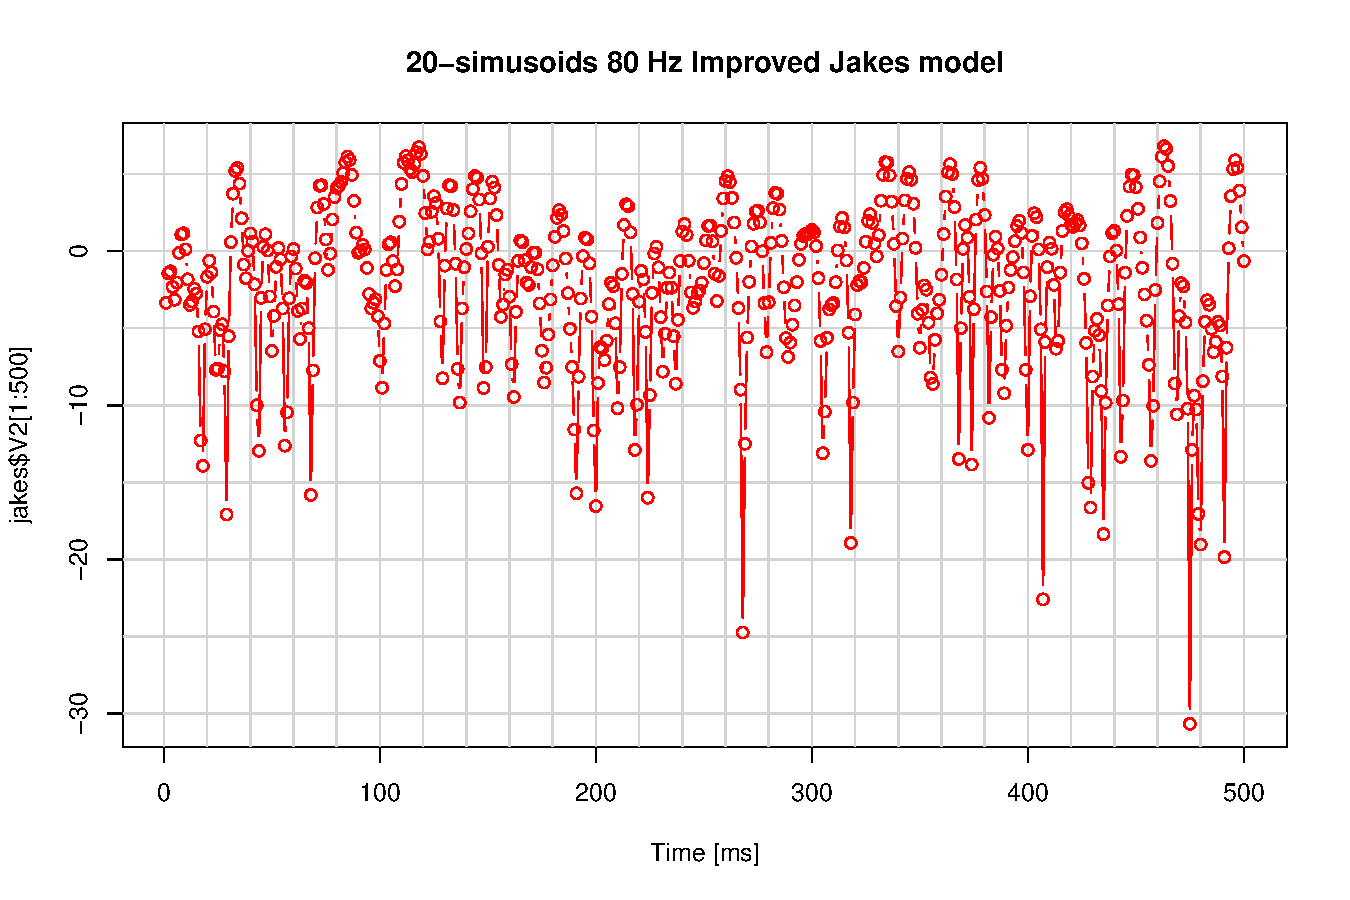
\includegraphics[width=1.1\textwidth]{pics/jakes-main.pdf}
\end{frame}
%--------------------------------------------------------------------------------
%--------------------------------------------------------------------------------
\begin{frame}
\frametitle{Пример}
\centering
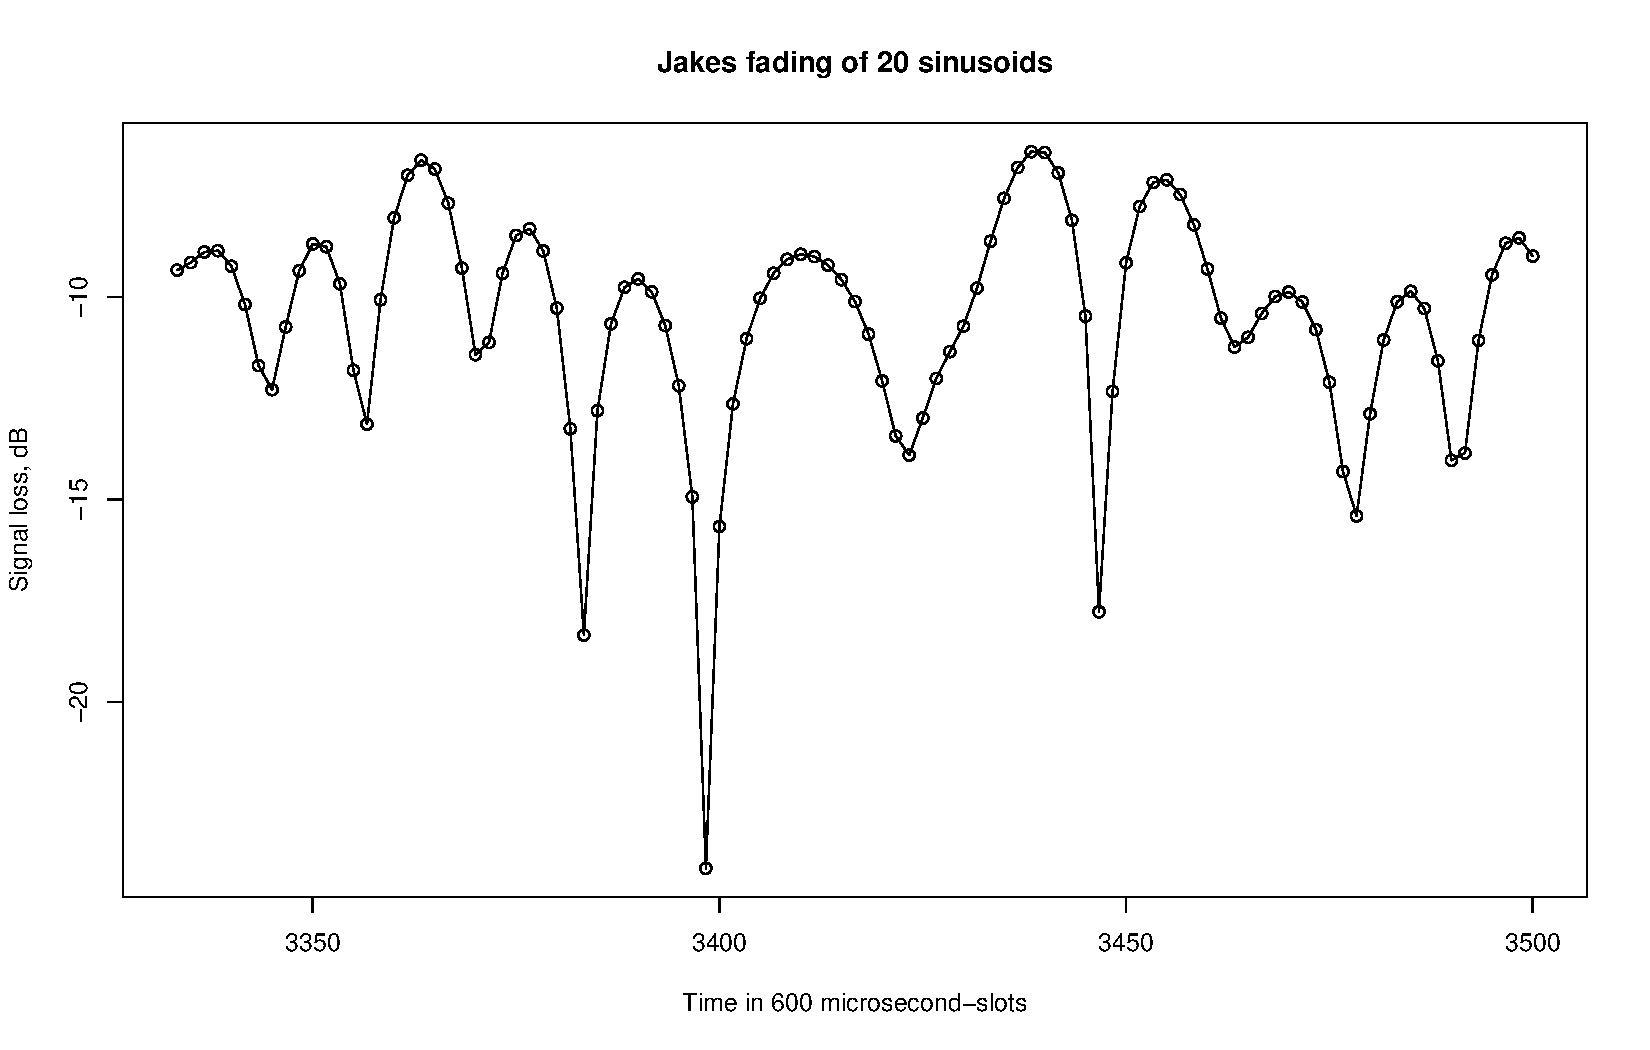
\includegraphics[width=1.1\textwidth]{pics/jakes-zoom.pdf}
\end{frame}
%--------------------------------------------------------------------------------
\begin{frame}
\frametitle{Широкополосный Рэлеевский беспроводной канал}
\centering
\includegraphics[width=1.1\textwidth]{pics/wideband-rayleigh.pdf}
\begin{itemize}
 \item Power Delay Profile -- характеризует частотную характеристику $e^{\frac{-t}{\tau}}$
 \item Каждый отсчёт сигнала характеризуется узкополосным Доплеровским случайным процессом
\end{itemize}
\end{frame}
%--------------------------------------------------------------------------------
\end {document}
